% Font options: 10pm, 11pt, 12pt
% Align headings left instead of center: nocenter
\documentclass[xcolor=x11names,compress]{beamer}\usepackage[]{graphicx}\usepackage[]{color}
%% maxwidth is the original width if it is less than linewidth
%% otherwise use linewidth (to make sure the graphics do not exceed the margin)
\makeatletter
\def\maxwidth{ %
  \ifdim\Gin@nat@width>\linewidth
    \linewidth
  \else
    \Gin@nat@width
  \fi
}
\makeatother

\definecolor{fgcolor}{rgb}{0.345, 0.345, 0.345}
\newcommand{\hlnum}[1]{\textcolor[rgb]{0.686,0.059,0.569}{#1}}%
\newcommand{\hlstr}[1]{\textcolor[rgb]{0.192,0.494,0.8}{#1}}%
\newcommand{\hlcom}[1]{\textcolor[rgb]{0.678,0.584,0.686}{\textit{#1}}}%
\newcommand{\hlopt}[1]{\textcolor[rgb]{0,0,0}{#1}}%
\newcommand{\hlstd}[1]{\textcolor[rgb]{0.345,0.345,0.345}{#1}}%
\newcommand{\hlkwa}[1]{\textcolor[rgb]{0.161,0.373,0.58}{\textbf{#1}}}%
\newcommand{\hlkwb}[1]{\textcolor[rgb]{0.69,0.353,0.396}{#1}}%
\newcommand{\hlkwc}[1]{\textcolor[rgb]{0.333,0.667,0.333}{#1}}%
\newcommand{\hlkwd}[1]{\textcolor[rgb]{0.737,0.353,0.396}{\textbf{#1}}}%
\let\hlipl\hlkwb

\usepackage{framed}
\makeatletter
\newenvironment{kframe}{%
 \def\at@end@of@kframe{}%
 \ifinner\ifhmode%
  \def\at@end@of@kframe{\end{minipage}}%
  \begin{minipage}{\columnwidth}%
 \fi\fi%
 \def\FrameCommand##1{\hskip\@totalleftmargin \hskip-\fboxsep
 \colorbox{shadecolor}{##1}\hskip-\fboxsep
     % There is no \\@totalrightmargin, so:
     \hskip-\linewidth \hskip-\@totalleftmargin \hskip\columnwidth}%
 \MakeFramed {\advance\hsize-\width
   \@totalleftmargin\z@ \linewidth\hsize
   \@setminipage}}%
 {\par\unskip\endMakeFramed%
 \at@end@of@kframe}
\makeatother

\definecolor{shadecolor}{rgb}{.97, .97, .97}
\definecolor{messagecolor}{rgb}{0, 0, 0}
\definecolor{warningcolor}{rgb}{1, 0, 1}
\definecolor{errorcolor}{rgb}{1, 0, 0}
\newenvironment{knitrout}{}{} % an empty environment to be redefined in TeX

\usepackage{alltt}
%\documentclass[xcolor=x11names,compress,handout]{beamer}
\usepackage[]{graphicx}
\usepackage[]{color}
\usepackage{booktabs}
\usepackage{hyperref}
\usepackage{tikz}
\usepackage{multirow}
\usepackage{dcolumn}
\usepackage{bigstrut}
\usepackage{amsmath} 
\usepackage{xcolor,colortbl}
\usepackage{amssymb}
%\newcommand{\done}{\cellcolor{teal}#1}

%% Beamer Layout %%%%%%%%%%%%%%%%%%%%%%%%%%%%%%%%%%
\useoutertheme[subsection=false,shadow]{miniframes}
\useinnertheme{default}
\usefonttheme{serif}
\usepackage{Arev}
\usepackage{pdfpages}
\usepackage[normalem]{ulem}

\setbeamerfont{title like}{shape=\scshape}
\setbeamerfont{frametitle}{shape=\scshape, size=\normalsize}

\definecolor{dkblue}{RGB}{0,0,102}

\setbeamercolor*{lower separation line head}{bg=dkblue} 
\setbeamercolor*{normal text}{fg=black,bg=white} 
\setbeamercolor*{alerted text}{fg=red} 
\setbeamercolor*{example text}{fg=black} 
\setbeamercolor*{structure}{fg=black} 
 
\setbeamercolor*{palette tertiary}{fg=black,bg=black!10} 
\setbeamercolor*{palette quaternary}{fg=black,bg=black!10} 

\renewcommand{\(}{\begin{columns}}
\renewcommand{\)}{\end{columns}}
\newcommand{\<}[1]{\begin{column}{#1}}
\renewcommand{\>}{\end{column}}

\setbeamertemplate{navigation symbols}{} 
\setbeamertemplate{footline}[frame number]
\setbeamertemplate{caption}{\raggedright\insertcaption\par}

\setbeamersize{text margin left=5pt,text margin right=5pt}

%%%%%%%%%%%%%%%%%%%%%%%%%%%%%%%%%%%%%%%%%%%%%%%%%%




\title{Making Causal Critiques}
\subtitle{Day 1 - Deconstructing an Argument}
\author{Jonathan Phillips}
\IfFileExists{upquote.sty}{\usepackage{upquote}}{}
\begin{document}

\frame{\titlepage}

\section{Introduction}

\begin{frame}
\frametitle{Causal Critiques}
\begin{itemize}
\item Political science is about \textit{explaining} outcomes
\begin{itemize}
\item Do parliamentary systems last longer than presidential ones?
\item Does development lead to democracy?
\item Does democracy prevent war?
\item Did voters support President Trump because of jobs lost to immigration?
\end{itemize}
\end{itemize}

\end{frame}

\begin{frame}
\frametitle{Causal Critiques}
\begin{itemize}
\item What is a causal critique?
\end{itemize}
\begin{table}[htbp]
  \centering
    \begin{tabular}{|>{\raggedright}p{5cm}|p{5cm}|}
    \hline
    Do parliamentary systems last longer than presidential ones? & "No, Parliamentary systems last longer because they are in Europe, not because they are parliamentary" \pause \\
    \hline
    Does development lead to democracy? & "No, democracy causes development" \pause \\
    \hline
    Does democracy prevent war? & "Of course not, India and Pakistan were democracies and had a war in 1999" \pause \\
    \hline
    Did voters support President Trump because of jobs lost to immigration? & "Obviously not, jobs were lost to technological change" \\
    \hline
    \end{tabular}%
  \label{tab:addlabel}%
\end{table}%
\end{frame}

\begin{frame}
\frametitle{Causal Critiques}
\begin{itemize}
\item What is a causal critique?
\begin{itemize}
\item A comment at a seminar
\item A critique of a policy
\item A response as a journal referee
\item Advice to a friend
\item A worry about your own research paper
\end{itemize}
\end{itemize}
\end{frame}

\begin{frame}
\frametitle{What makes an Argument?}
\begin{itemize}
\item  Explanation requires:
\begin{enumerate}
\item  Evidence
\item  Theory
\end{enumerate}
\end{itemize}
\end{frame}

\begin{frame}
\frametitle{What makes an Argument?}
\begin{itemize}
\item Why does a ball always fall downwards?
\begin{itemize}
\item What is the evidence?
\pause
\item What is the theory?
\end{itemize}
\end{itemize}
\end{frame}

\begin{frame}
\frametitle{What makes an Argument?}
\begin{itemize}
\item Why does a ball always fall downwards?
\item Evidence can be:
\begin{itemize}
\item \textbf{Quantitative}: We take a series of numeric measurements of the direction of the ball's travel
\item \textbf{Qualitative}: We observe or ask people about the direction of the ball's travel
\end{itemize}
\item But the same \textbf{Logic of Inference} applies to both
\begin{itemize}
\item We want to gather information to reliably evaluate if a theory is correct
\item Our conclusions are always uncertain, but we want to limit the uncertainty
\end{itemize}
\end{itemize}
\end{frame}

\section{Logical Consistency}

\begin{frame}
\frametitle{What makes an Argument Convincing?}
\begin{itemize}
\item To be good causal explanations, theories need to be \textbf{logically consistent}
\begin{itemize}
\item All policemen wear hats. This person is a policeman. Therefore this person is wearing a hat.
\item $\forall p:  h, p \Rightarrow h$
\end{itemize}
\end{itemize}
\end{frame}

\begin{frame}
\frametitle{What makes an Argument Convincing?}
\begin{itemize}
\item To be good causal explanations, theories need to be \textbf{logically consistent}
\begin{itemize}
\item All policemen wear hats. This person is wearing a hat. Therefore this person is a policeman.
\item $\text{\sout{\ensuremath{\forall p:  h, \Rightarrow p}}}$
\end{itemize}
\end{itemize}
\end{frame}

\begin{frame}
\frametitle{What makes an Argument Convincing?}
\begin{itemize}
\item Logical Fallacies
\begin{enumerate}
\item \textbf{False syllogism}: Conclusions do not follow from premises
\begin{itemize}
\item Eg. Some cats are black. Some black things are televisions. Therefore some cats are televisions.
\end{itemize}
\item \textbf{False dichotomy}: Restricting the possible options to only two
\begin{itemize}
\item Eg. "Either we attack them first or they attack us first"
\end{itemize}
\item \textbf{Circular reasoning}: The conclusions just restate the premises
\begin{itemize}
\item Eg. "Abortion should be legal because women have the right to an abortion."
\end{itemize}
\end{enumerate}
\end{itemize}
\end{frame}

\begin{frame}
\frametitle{What makes an Argument Convincing?}
\begin{itemize}
\item Logical Fallacies
\begin{enumerate}
\setcounter{enumi}{3}
\item \textbf{Over-generalization}: Extending the conclusions beyond the scope of the evidence
\begin{itemize}
\item Eg. "All of my friends support party X so of course they will win the election"
\end{itemize}
\item \textbf{Post hoc Fallacy}: Just because something happened earlier does not mean it was the cause
\begin{itemize}
\item Eg. "You moved into this apartment yesterday and now the cooker is broken. It must be your fault."
\end{itemize}
\item \textbf{Appeal to Authority}: Assuming the author is right because they are senior
\begin{itemize}
\item Eg. Assuming that political science professors know what they are doing!
\end{itemize}
\end{enumerate}
\end{itemize}
\end{frame}

\begin{frame}
\frametitle{What makes an Argument Convincing?}
\begin{itemize}
\item Does the introduction of mobile phone service reduce price variation in Kerala's fishing industry?
\begin{itemize}
\item Jensen et al 2007
\end{itemize}
\end{itemize}
\end{frame}

\setbeamercolor{background canvas}{bg=}
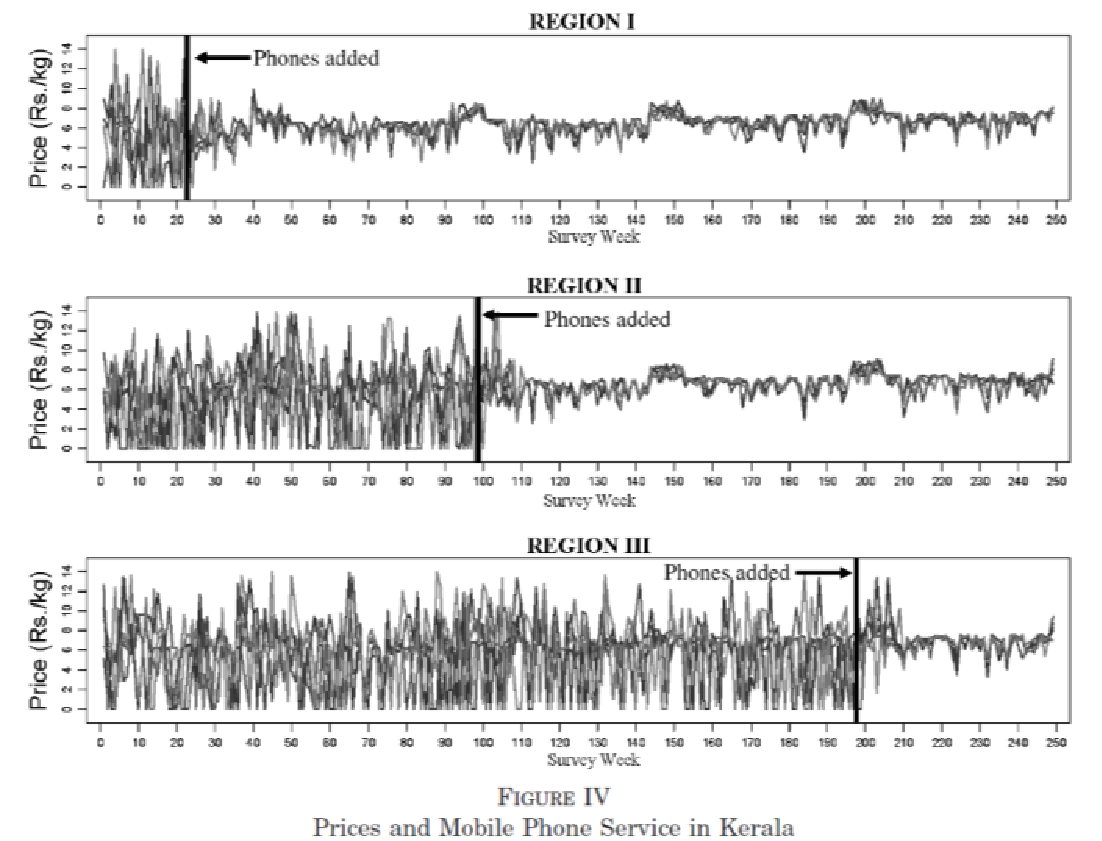
\includepdf[pages={1}]{Phone_Prices.pdf}

\begin{frame}
\frametitle{What makes an Argument Convincing?}
\begin{itemize}
\item Gathering evidence in political science is particularly hard:
\begin{enumerate}
\item Humans are complex and unpredictable, unlike the natural sciences
\item Societies are even more complex interactions of millions of humans
\item Everyone has an opinion, including researchers
\item Ethical constraints on the data we can gather
\item Political explanations in one place may not work in another
\end{enumerate}
\end{itemize}
\end{frame}

\section{Deconstructing Papers}

\begin{frame}
\frametitle{Deconstructing a Political Science Paper}
\begin{itemize}
\item Before we can critique an argument we have to understand its content
\begin{itemize}
\item What concepts it uses
\item How those concepts are measured
\item What theory connects the concepts
\item Where did the data come from?
\item What methodology produced the evidence?
\item What is the scope of the argument's application?
\end{itemize}
\end{itemize}
\end{frame}

\begin{frame}
\frametitle{Deconstructing a Political Science Paper}
\begin{itemize}
\item How to read a political science paper:
\begin{itemize}
\item Actively, intentionally
\item Not like a Harry Potter book!
\item Read the abstract, conclusion, charts many times
\item Look for keywords: "We can conclude that...", "Our argument is that..."
\item Make notes \textit{only} of what you have learnt
\item Summarize the paper in your own words
\end{itemize}
\end{itemize}
\end{frame}

\begin{frame}
\frametitle{Deconstructing a Political Science Paper}
\begin{itemize}
\item Elements of a political science paper:
\begin{itemize}
\item \textbf{Research question} - the authors are engaging with a specific literature/puzzle
\item \textbf{Answer/Causal argument} - "We argue that  increases Y"
\item \textbf{Scope of argument} - Does the argument apply only to democracies, Asian countries, since World War II, only to women?
\end{itemize}
\end{itemize}
\end{frame}

\begin{frame}
\frametitle{Deconstructing a Political Science Paper}
\begin{itemize}
\item Elements of a political science paper:
\begin{itemize}
\item \textbf{Concepts/Variables} - What political factors do the authors think matter?
\item \textbf{Measures} - What political factors do the authors actually measure?
\item \textbf{Units of Analysis} - At what level are these measures taken; individuals, countries, city-years?
\item \textbf{Role of Variables} - Which is the outcome variable and which the explanatory? What controls are used?
\end{itemize}
\end{itemize}
\end{frame}

\begin{frame}
\frametitle{Deconstructing a Political Science Paper}
\begin{itemize}
\item Elements of a political science paper:
\begin{itemize}
\item \textbf{Theory} - What social, economic or psychological process links the explanatory and outcome variables? 
\item \textbf{Methodology} - What strategy do the authors use to gather evidence to evaluate the theory?
\item \textbf{Evidence} - What evidence does the methodology produce?
\end{itemize}
\end{itemize}
\end{frame}

\begin{frame}
\frametitle{Deconstructing a Political Science Paper}
\begin{itemize}
\item Methodology is crucial
\item Where did the dataset come from?
\begin{itemize}
\item Sampling strategy
\item Questionnaire and survey protocol
\item Measurement error
\item Data entry, cleaning
\item Statistics/statistical model chosen
\end{itemize}
\item How does this data help us answer the question?
\end{itemize}
\end{frame}

\begin{frame}
\frametitle{Deconstructing a Political Science Paper}
\begin{itemize}
\item Methodologies for gathering evidence:
\item Observational Studies:
\begin{itemize}
\item Case Study, Process Tracing
\item Comparative Cases
\item Regression with controls
\item Matching
\end{itemize}
\end{itemize}
\end{frame}

\begin{frame}
\frametitle{Deconstructing a Political Science Paper}
\begin{itemize}
\item Methodologies for gathering evidence:
\item Experimental Studies:
\begin{itemize}
\item Field Experiment
\item Lab/Survey Experiment
\end{itemize}
\end{itemize}
\end{frame}

\begin{frame}
\frametitle{Deconstructing a Political Science Paper}
\begin{itemize}
\item Methodologies for gathering evidence:
\item Quasi-Experimental Studies:
\begin{itemize}
\item Natural Experiment
\item Instrumental Variable
\item Regression Discontinuity
\item Difference-in-Differences
\end{itemize}
\end{itemize}
\end{frame}

\setbeamercolor{background canvas}{bg=}
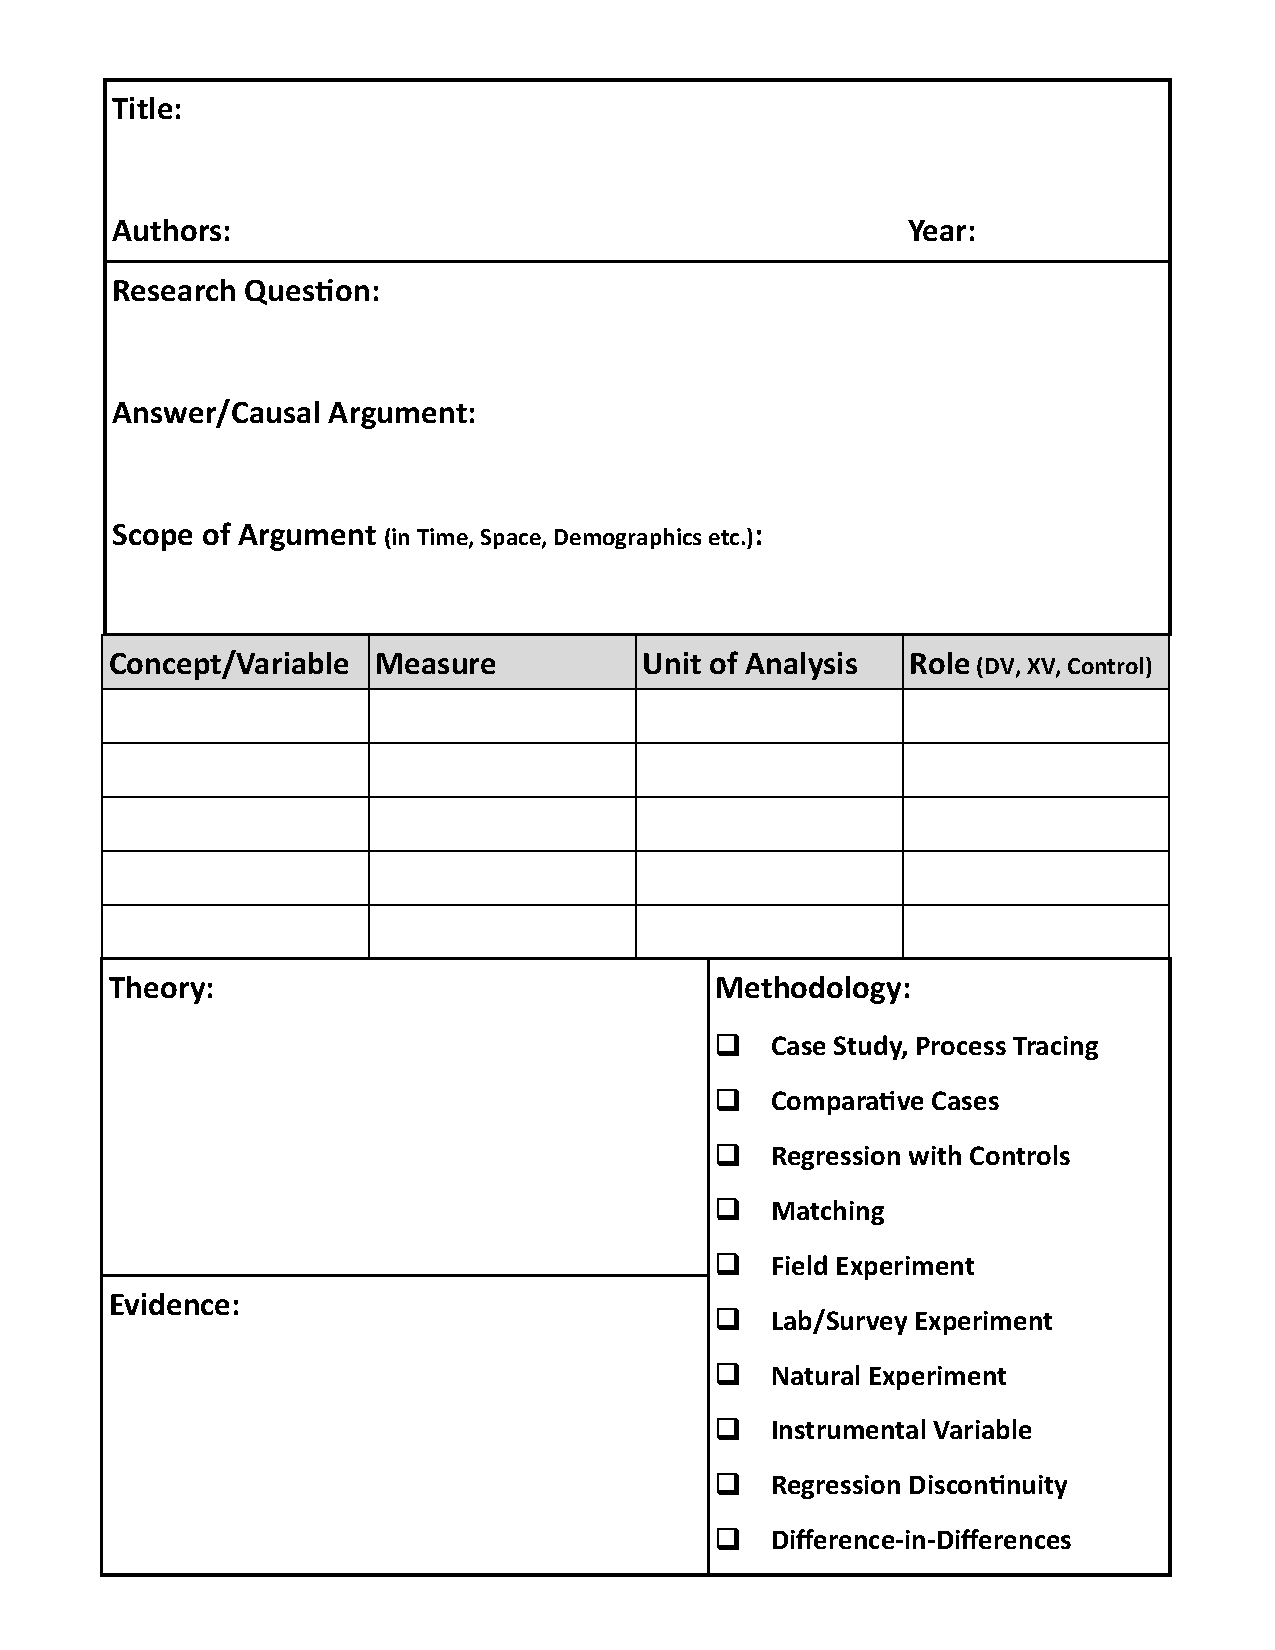
\includepdf[pages={1}]{Paper_summary_template.pdf}

\setbeamercolor{background canvas}{bg=}
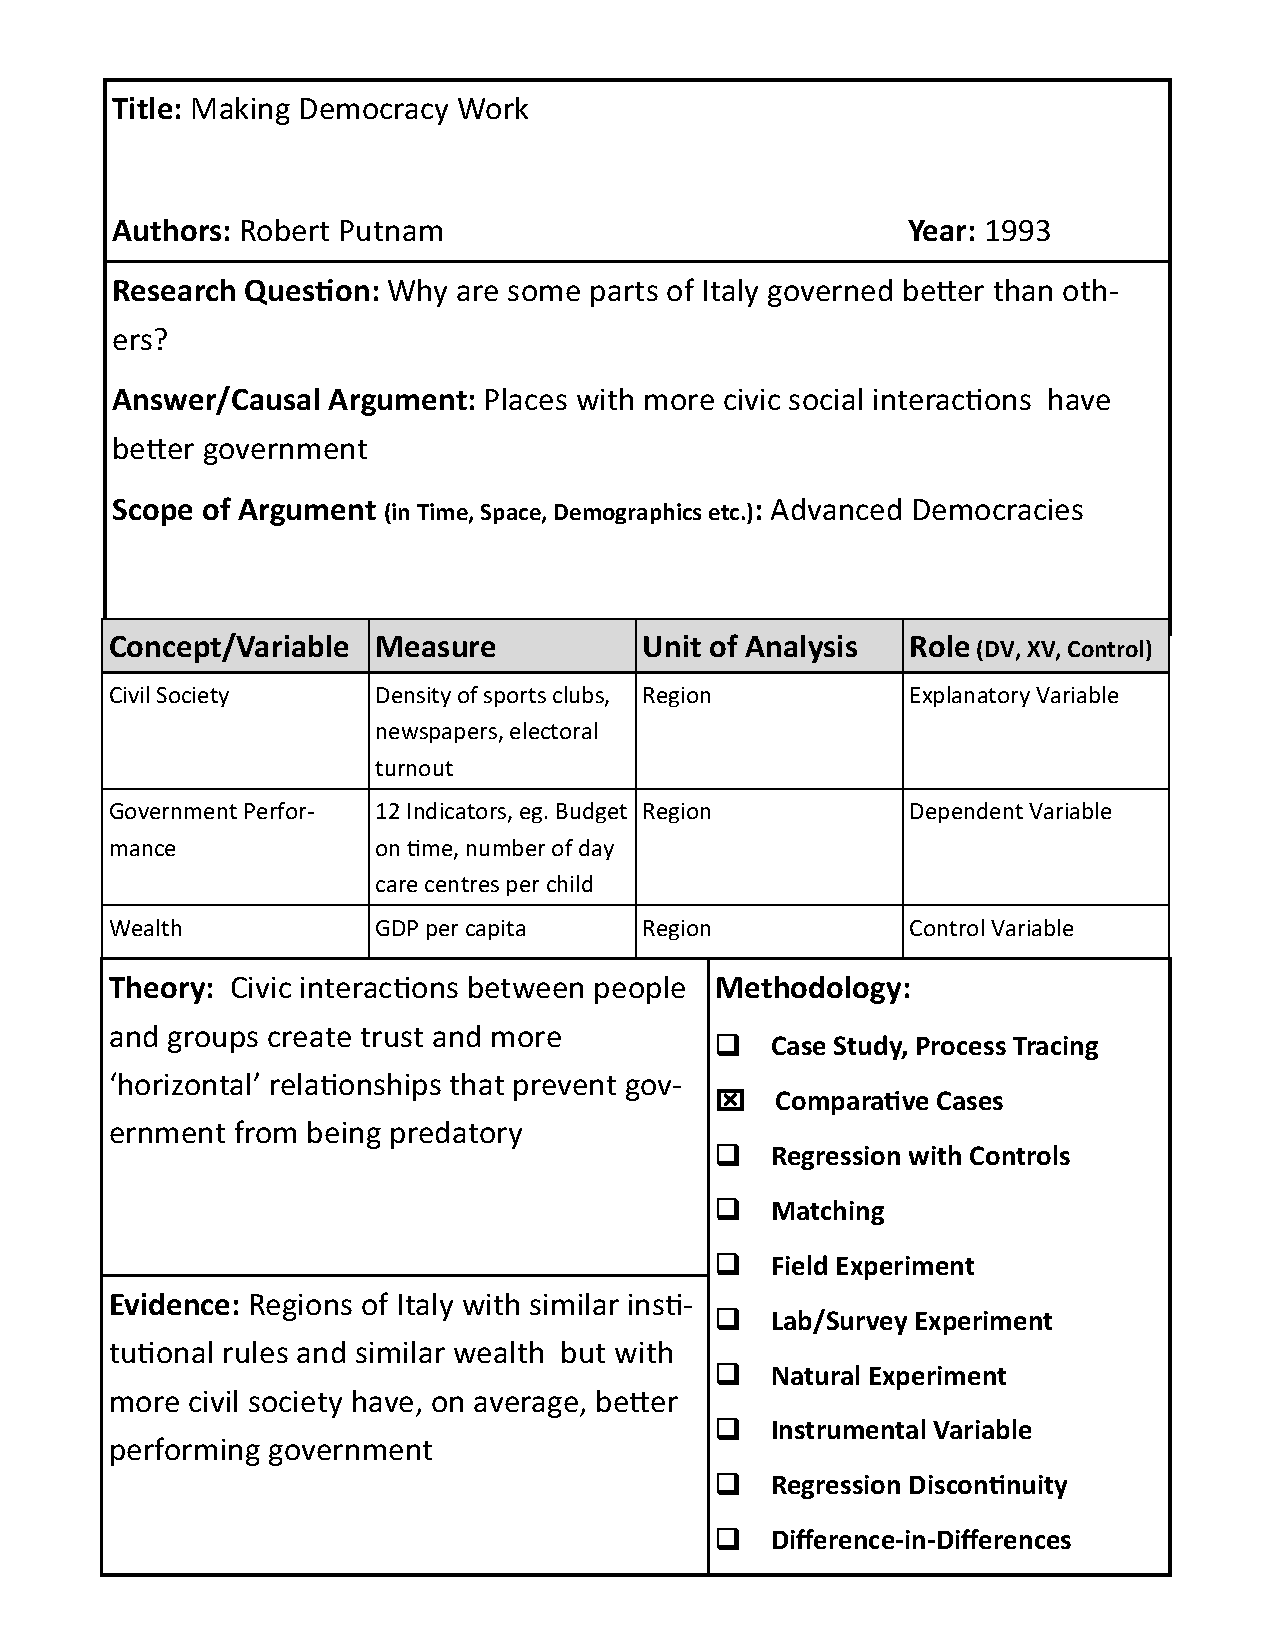
\includepdf[pages={1}]{Paper_summary_template_Putnam.pdf}

\begin{frame}
\frametitle{Deconstructing a Political Science Paper}
\begin{itemize}
\item Using Causal Diagrams to clarify arguments
\item Technically, "Directed Acyclical Graphs" (DAGs)
\begin{itemize}
\item Write all the variables on the paper
\item Connecting them with arrows to represent the author's \textbf{causal} argument
\item And also the \textit{threats} to the author's argument
\begin{itemize}
\item Even if they can't be measured
\end{itemize}
\end{itemize}
\end{itemize}
\end{frame}

\begin{frame}
\frametitle{Deconstructing a Political Science Paper}
\begin{knitrout}
\definecolor{shadecolor}{rgb}{0.969, 0.969, 0.969}\color{fgcolor}
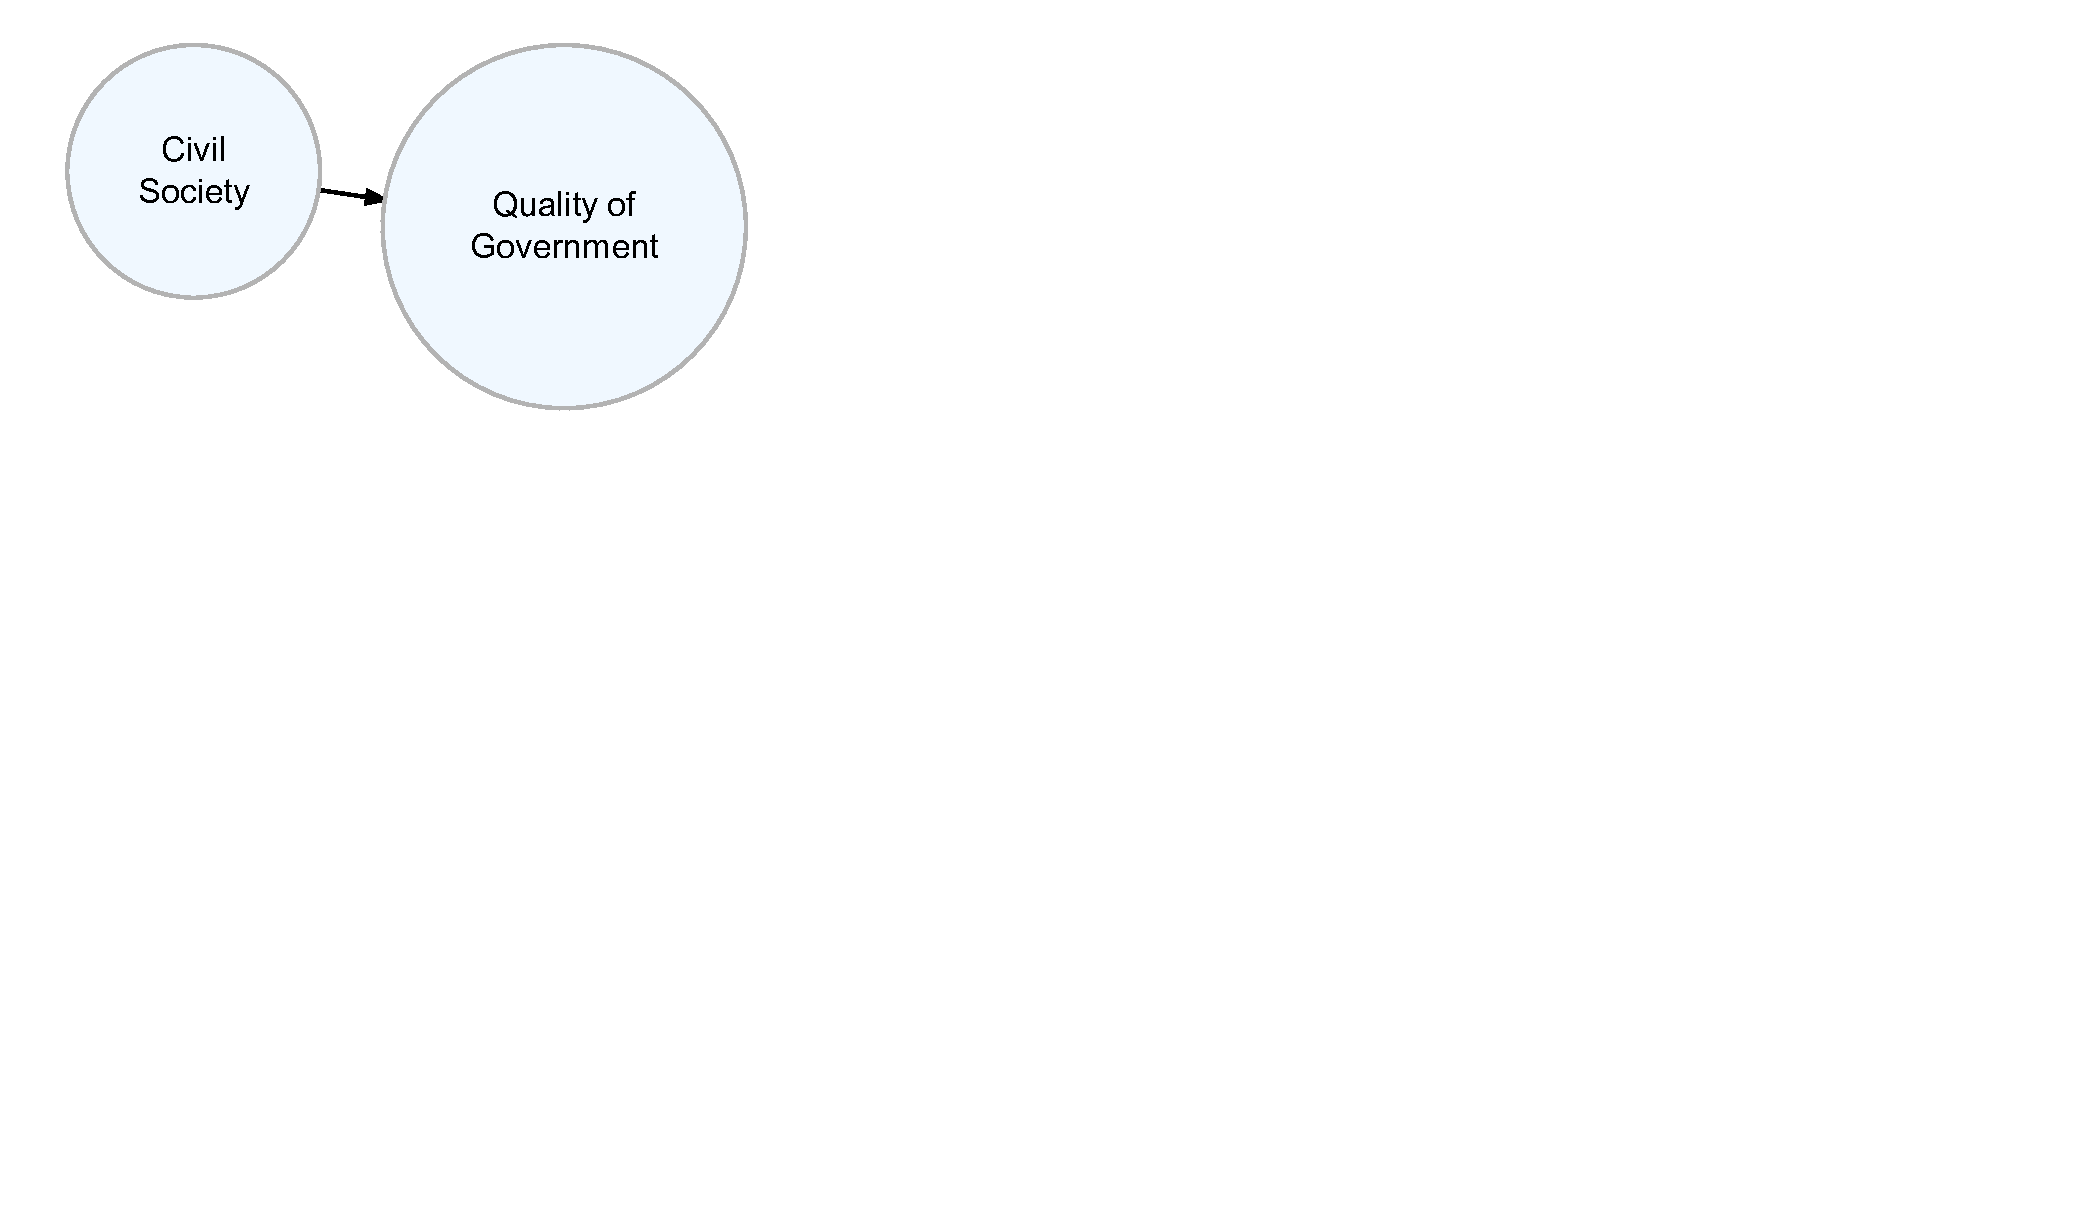
\includegraphics[width=\maxwidth]{figure/unnamed-chunk-1-1} 

\end{knitrout}
\end{frame}

\begin{frame}
\frametitle{Deconstructing a Political Science Paper}
\begin{knitrout}
\definecolor{shadecolor}{rgb}{0.969, 0.969, 0.969}\color{fgcolor}
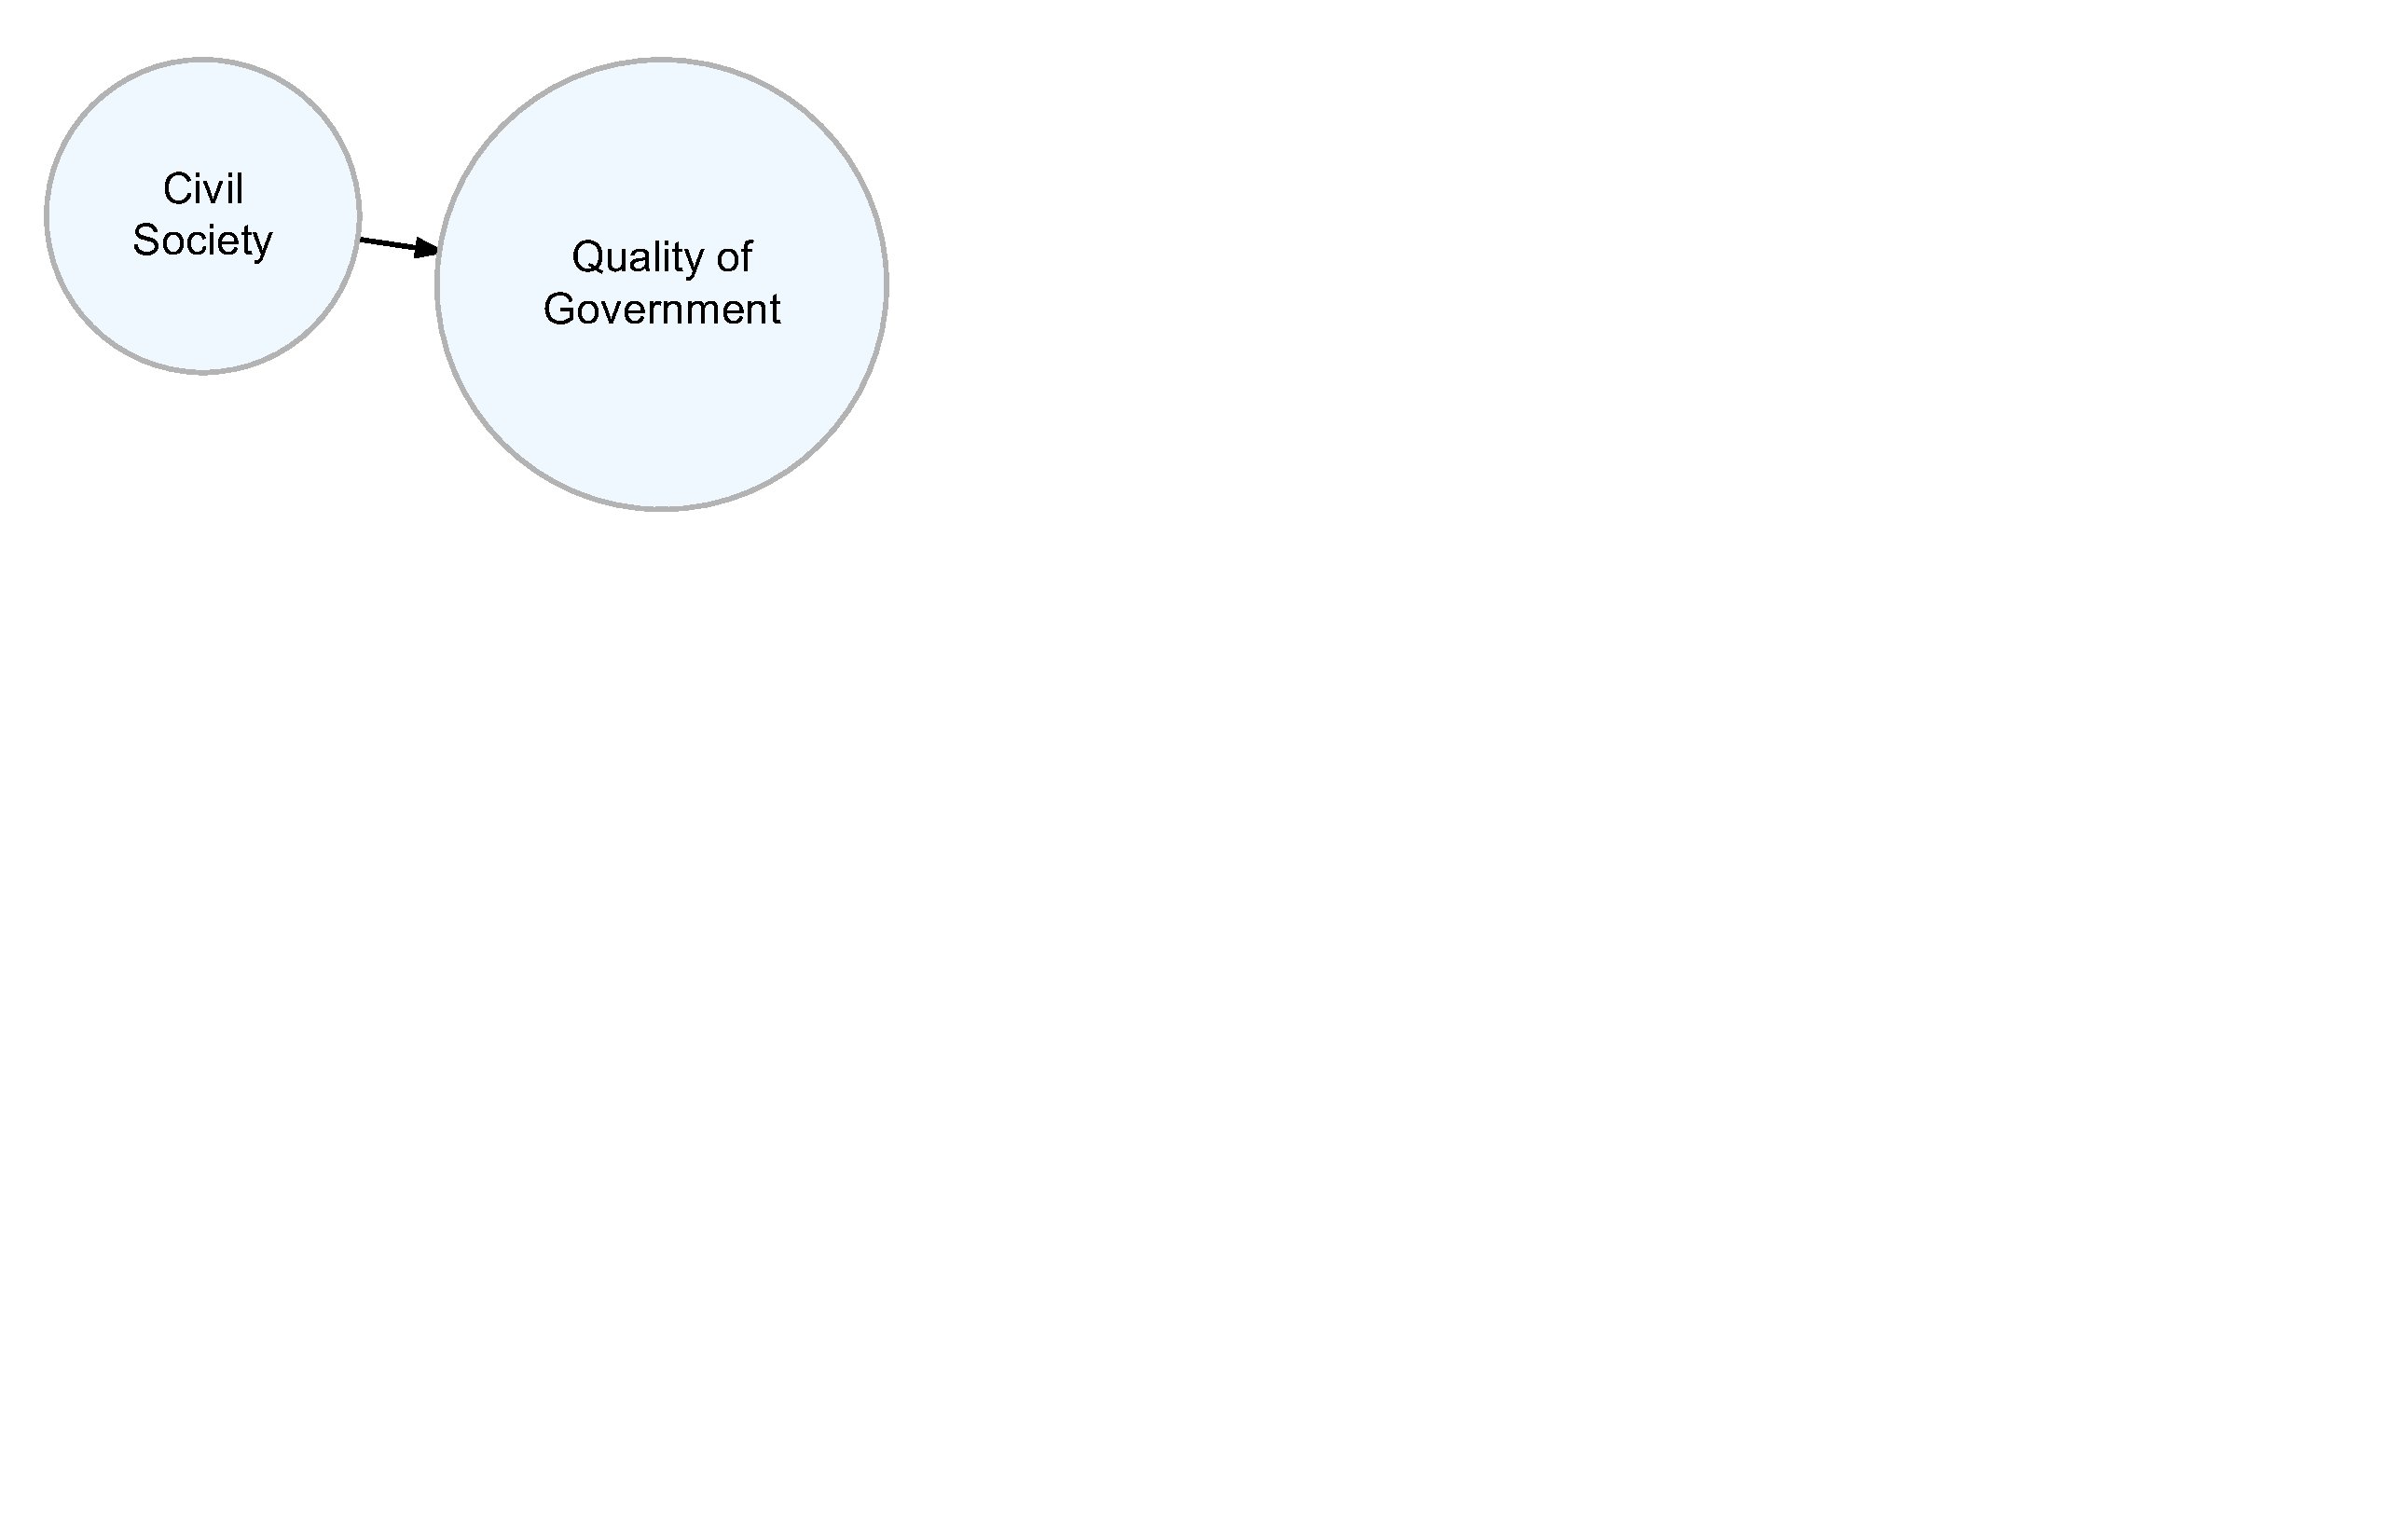
\includegraphics[width=\maxwidth]{figure/unnamed-chunk-2-1} 

\end{knitrout}
\end{frame}

\begin{frame}
\frametitle{Types of Causation}
\begin{enumerate}
\item \textbf{Deterministic Causation} - If $x$ then $y$
\item \textbf{Probabilistic Causation} - If $x$ then the probability of $y$ increases
\item \textbf{Conjuctural Causation} - If $x1$ and $x2$ then $y$
\item \textbf{Equifinality Causation} - If $x1$ or $x2$ then $y$
\item \textbf{Non-Linear Causation} - If $x>1000$ then $y$
\item \textbf{Path-Dependent Causation} - If $x$ and $t=10$ then $y$
\item \textbf{Granger Causation} - If $x$ before $y$, $x$ causes $y$
\end{enumerate}
\end{frame}


%%Types of Explanation

\begin{frame}
\frametitle{What makes a Good Causal Argument? (Gerring 2005)}
\begin{enumerate}
\item \textbf{Specificity} - Is the argument clear and internally consistent?
\item \textbf{Parsimony} - Is the argument simple?
\item \textbf{Power} - How much does $y$ change?
\item \textbf{Precision} - How much uncertainty is there about how much $y$ changes?
\item \textbf{Scope} - What is the breadth of conditions under which the effect occurs
\item \textbf{Differentiation} - Is the $x$ sufficiently different from the $y$
\item \textbf{Normality} - Is $x$ a common event?
\item \textbf{Mechanism} - Do we understand what connects $x$ to $y$?
\item \textbf{Consistency} - Is the argument consistent with our other knowledge about the world?
\item \textbf{Policy-relevance} - Can the argument help us design better policy?
\end{enumerate}
\end{frame}

\begin{frame}
\frametitle{What makes a Good Causal Argument? (Gerring 2005)}
\begin{itemize}
\item Evaluate these causal arguments based on the above criteria:
\begin{itemize}
\item Every extra \$1000 of income per person makes democracy 10\% more stable, +/-8%
\item Tall presidents are more successful
\item Non-African countries with open-list proportional representation in the Southern hemisphere always pass their budgets late
\end{itemize}
\end{itemize}
\end{frame}

\begin{frame}
\frametitle{What makes Good Causal Evidence? (Gerring 2005)}
\begin{enumerate}
\item \textbf{Sample Size} - How many cases are we learning from?
\item \textbf{Variation} - Do the causes and outcomes really vary in the sample?
\item \textbf{Representative} - Does the sample reflect the population?
\item \textbf{Independence} - Are the observations clustered (and therefore less useful)?
\item \textbf{Comparability} - Are the units of the same type?
\item \textbf{Transparency} - Do the data tell us about the mechanism connecting $x$ and $y$?
\item \textbf{Replicability} - Can we take the same (or similar) data and reach the same conclusion?
\end{enumerate}
\end{frame}

\begin{frame}
\frametitle{What makes Good Causal Evidence? (Gerring 2005)}
\begin{itemize}
\item Evaluate this causal evidence based on the above criteria:
\begin{itemize}
\item 30 interviews with male politicians in Iraq to understand whether education levels affects how they govern
\item Analysis of secondary data from Africa to understand if drought (measured as rainfall/$km^2$) causes more violence (measured as number of terrorist attacks)
\item Representative household survey of 20,000 Mexican voters to assess whether perceptions of the economy affect voting behaviour
\end{itemize}
\end{itemize}
\end{frame}


\begin{frame}
\frametitle{Fundamental Critiques}
\begin{itemize}
\item 
\item \textbf{Conceptual Validity} - Competitive authoritarianism vs. Illiberal Democracy
\begin{itemize}
\item Avoid conceptual stetching!
\item We can move "up and down the ladder of generality" (Sartori)
\end{itemize}
\item \textbf{Measurement Validity} - when scores "meaningfully capture the ideas contained in the corresponding concept"
\begin{itemize}
\item Does the scale make sense? Is democracy binary or continuous?
\item Are the cases (units) scored correctly? How reliable is the scoring?
\end{itemize}
\end{itemize}
\end{frame}

\setbeamercolor{background canvas}{bg=}
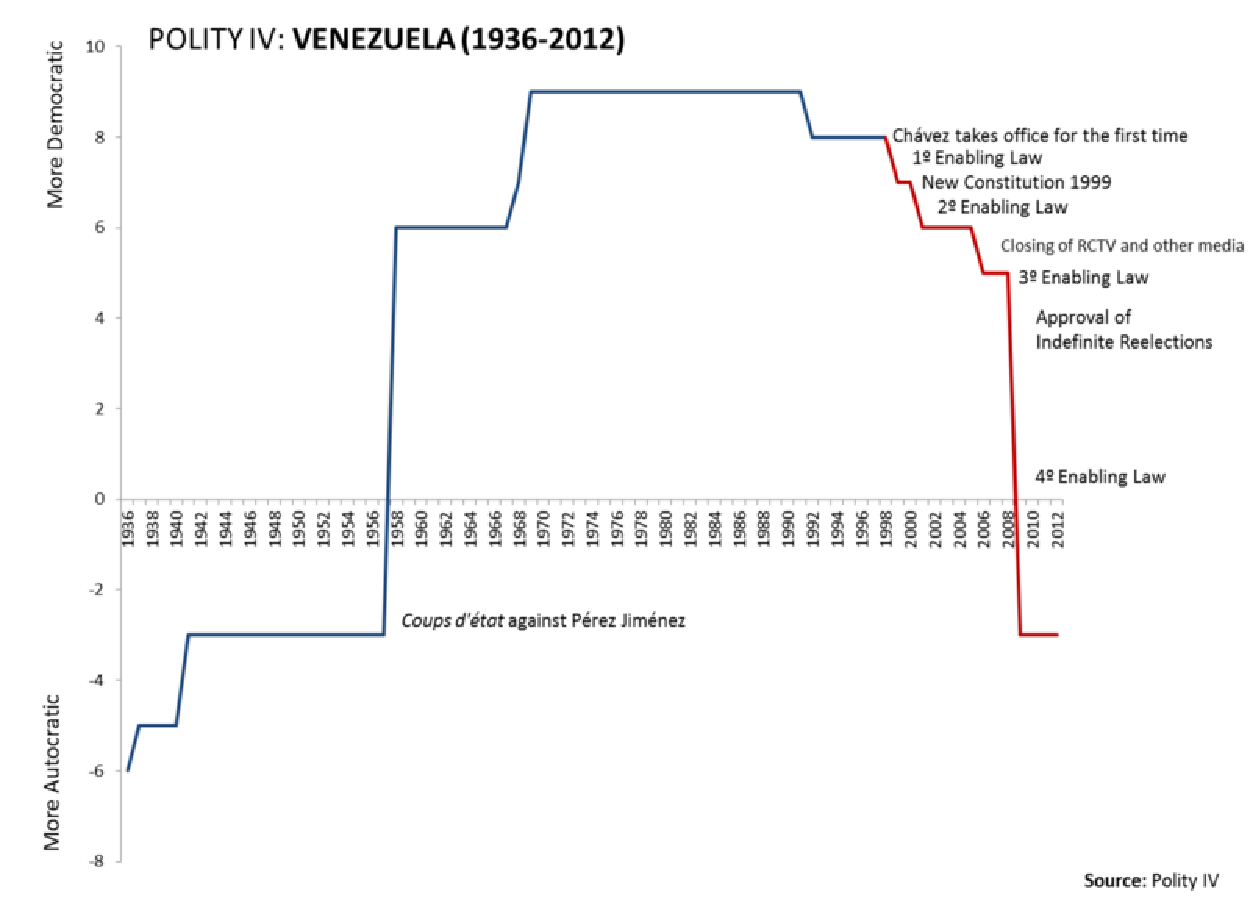
\includepdf[pages={1}]{Polity.pdf}

\end{document}
 
 % effects of causes vs. reverse
